\chapter{Conclusiones y trabajo futuro}
\label{conclusiones}

 En este capítulo, se finalizará la memoria con las conclusiones del trabajo realizado, haciendo una valoración del mismo y de los resultados obtenidos del desarrollo. Además, se presentarán las vías de trabajo futuro que han ido apareciendo a medida que se realizaba el \gls{tfg}. En concreto, se expondrán dichas vías, y se concluirá con un breve análisis sobre la viabilidad de las mismas.
%%%%%%%%%%%%%%%%%%%%%%%%%%%%%%%%%%%%%%%%%%%%%%%%%%%%%%%%%%%%%%%%%%%%%%%%%%%%%%%%%%%%%%%%%%%%%%%%%
\section{Conclusiones del \glsentryshort{tfg}}

La finalidad de los casos de uso era la de ver con qué tecnología (\gls{xdp}, P4) es más sencillo y eficiente definir el \textit{datapath} de los dispositivos \gls{iot} en entornos \gls{sdn}. Por tanto, antes de realizar las conclusiones, se deberá revisar los resultados de las evaluaciones de ambas tecnologías en los distintos entornos, cableado e inalámbrico. \\
\par
Como se puede apreciar en la tabla \ref{tab:useCases}, con la tecnología \gls{xdp} en medios cableados no se pudo realizar un Broadcast de forma nativa, es decir, dicha tecnología no fue suficiente para lograr el broadcast. Es verdad que dicha limitación fue estudiada, y se planteó una solución, haciendo uso de un programa \gls{bpf} adicional en el \gls{tc}, pero aún teniendo en cuenta que se solucionó, no se puede afirmar que la tecnología lo soporte.  En cambio, si se observa dicha funcionalidad en un entorno Wireless, ya no habría dicha limitación dado que no sería necesario clonar los paquetes. Generalmente cambiando la dirección destino del paquete de capa dos a difusión, y transmitiéndolo al medio, será suficiente para lograr el Broadcast. \\
\par



En cambio, la tecnología P4, a diferencia de \gls{xdp}, tiene una interfaz de alto nivel para definir funcionalidades de broadcast/multicast. Esta interfaz, comúnmente conocida como ``grupos multicast", permite definir en una estructura de datos de tipo JSON por qué puertos inundar y con qué cantidad de réplicas por puerto. De forma adicional, cabe mencionar que los grupos multicast permiten modificar el tipo de instancia de los paquetes clonados, siendo posible diferenciar los paquetes originales de los clonados. \\
\par

\begin{table}[ht]
\centering
\begin{tabular}{|l|c|c|c|c|}
\hline
\rowcolor[HTML]{EFEFEF} 
\multicolumn{1}{|c|}{\cellcolor[HTML]{EFEFEF}\textbf{Caso de uso}} & \textbf{XDP} & \textbf{P4} & \textbf{P4-Wireless} & \textbf{XDP-Wireless} \\ \hline
case01 - Drop                                                      & \cmark       & \cmark      & \cmark               & \cmark                \\ \hline
case02 - Pass                                                      & \cmark       & \xmark      & \xmark               & \cmark                \\ \hline
case03 - Echo server                                               & \cmark       & \cmark      & \cmark               & \cmark                \\ \hline
case04 - Layer 3 forwarding                                        & \cmark       & \cmark      & \cmark               & \cmark                \\ \hline
case05 - Broadcast                                                 & \xmark       & \cmark      & \cmark               & \cmark                \\ \hline
\end{tabular}
\caption{Resumen sobre los casos de uso desarrollados}
\label{tab:useCases}
\end{table}

Volviendo a la tabla \ref{tab:useCases}, se quiere hacer especial hincapié en que la tecnología P4 no soporta la funcionalidad de dejar pasar o delegar los paquetes, sin afectarles el plano de datos programado en P4. Por otro lado, con \gls{xdp} siempre se puede pasar el paquete al Kernel para que se encargue él del procesamiento. Sin embargo, en P4, se debe definir de forma exclusiva todo el \textit{datapath}, por lo que no hay a quien delegar el paquete, es decir, se tiene que encargar el propio programa P4. Este punto es muy positivo para \gls{xdp}, ya que acciones sencillas y repetitivas pueden ser definidas en un programa \gls{xdp} y delegar el resto de funcionalidades al Kernel. Por tanto, se actuaría de forma cooperativa y ganando en rendimiento como se vio en el case04 (\ref{xdp_ether_case04}), donde se trabajaba de forma conjunta para obtener información de routing desde el propio Kernel. \\
\par
Por último, se quiere mencionar la diferencia que existe entre ambas tecnologías en la interfaz de control. En P4 la interfaz de control serán las tablas, las cuales se definirán su estructura desde el propio programa P4 pero se irán completando vía P4Runtime por un controlador externo. Por ejemplo, ONOS\footnote{\url{https://wiki.onosproject.org/display/ONOS/P4+brigade}}, el cual soporta la configuración vía P4Runtime. En cambio, en \gls{xdp} se podría decir que el equivalente a las tablas serían los mapas \gls{bpf}.\\
\par
Estos mapas, de tipo clave-valor, son definidos por el programa que se ancla en el Kernel, y generalmente son completados por programas de espacio de usuario, que acceden a éste a través de descriptores de archivo. Se podría decir que es un sistema al que aún le queda recorrido para ser igual de consistente que las tablas en P4, dado que sería necesario el desarrollo de un servidor \gls{xdp} de espacio de usuario que estuviera a la escucha de información de control. Este servidor se encargaría de escribir en los mapas \gls{bpf} la información equivalente de control que permitiese que el programa anclado en el Kernel actuara acorde a las directrices de un hipotético controlador.\\
\par

Por tanto, se concluye indicando que la tecnología \gls{xdp} actualmente está mejor enfocada para escenarios de integración totales (Ver figura \ref{sdn_iot_total}), donde el dispositivo \gls{iot} únicamente dispone de interfaces wireless. Este dispositivo se beneficiará del rendimiento y la optimización de recursos que ofrece \gls{xdp} al actuar de forma reactiva a los paquetes. \\
\par
En cuanto a la tecnología P4 se cree que está más enfocada a escenarios de integración parcial (Ver figura \ref{sdn_iot_parcial}), donde el dispositivo \gls{iot} mediador dispone tanto de interfaces cableadas para comunicarse con el core \gls{sdn}, como de una interfaz inalámbrica para comunicarse con otros dispositivos \gls{iot}. Dichos dispositivos se beneficiarán de las facilidades que otorga P4 para realizar multicast, y de la interfaz de control tan bien definida que tiene para ser controlado por un controlador \gls{sdn} convencional.
\vspace{2cm}




\newpage
%%%%%%%%%%%%%%%%%%%%%%%%%%%%%%%%%%%%%%%%%%%%%%%%%%%%%%%%%%%%%%%%%%%%%%%%%%%%%%%%%%%%%%%%%%%%%%%%%
\section{Líneas de trabajo futuro}
\label{trabajoFuturo}

Como se ha podido apreciar a lo largo del \gls{tfg}, la tecnología \gls{xdp} aun se está asentando; se está abriendo camino dando nuevas posibilidades a los desarrolladores de la parte de \textit{Networking} del Kernel, reescribiendo herramientas y distintos procesos del \textit{stack} de red del Kernel de Linux\footnote{\url{https://github.com/xdp-project/net-next}}. Por otro lado, se encuentra la tecnología P4, la cual ya lleva un par de años en escena, pero cuya comunidad va aumentando día tras día,  con ello, la calidad y robustez de sus implementaciones.   \\
\par
Desgraciadamente, aunque estas dos tecnologías estén en constante crecimiento, no parece que a día de hoy haya un interés especial por llevarlas al \gls{iot}. Debido a lo cual, a lo largo de este \gls{tfg} no se ha encontrado la información suficiente, ni las plataformas adecuadas para realizar el estudio y análisis de la integración de los dispositivos \gls{iot} en entornos \gls{sdn}, llegando incluso a tener que realizar implementaciones personalizadas de plataformas para la emulación de redes wireless con finalidad de poder evaluar los casos de uso. \\
\par
El hecho que de que aún no haya un interés general por llevar a dichas tecnologías al mundo \gls{iot}, deja mucho por hacer, explorar, desarrollar y probar. A continuación, se indican las vías de trabajo futuro que se cree que abrirán el camino a futuros trabajos e implementaciones, que son principalmente dos: la manipulación directa de las cabeceras \texttt{ieee80211} y la evaluación en redes de baja capacidad (\texttt{ieee802154}).
%%%%%%%%%%%%%%%%%%%%%%%%%%%%%%%%%%%%%%%%%%%%%%%%%%%%%%%%%%%%%%%%%%%%%%%%%%%%%%%%%%%%%%%%%%%%%%%%%
\subsection{Integración de interfaces en modo monitor con los casos de uso}

Según lo explicado en el análisis de casos de uso inalámbricos, donde se hablaba sobre el módulo mac80211\_hwsim, al trabajar con dicho módulos terminamos haciendo uso de interfaces Ethernet que comunican con un radio \texttt{ieee80211}. Por tanto todos los paquetes que llegan a las interfaces llevan cabeceras Ethernet. Esto es debido a que en el Kernel se produce una traducción de cabeceras del estándar \texttt{ieee80211} al estándar \texttt{ieee8023}, y acto seguido se delegan los paquetes a la interfaz en cuestión. Para más información sobre este proceso de traducción se recomienda acudir al apartado \ref{limitacionesEncontradas} donde se explica con mayor detalle este proceso, a qué se debe, qué aporta y qué limitaciones induce al trabajar de esta manera.\\

\par
Debido a esta condición de diseño del módulo mac80211\_hwsim, no se ha podido gestionar de forma directa los paquetes con las cabeceras WiFi. Las interfaces creadas por este módulo, soportan varios modos de funcionamiento, y en el único modo de funcionamiento en el cual se puede llegar a ver las cabeceras WiFi es en el modo monitor, el cual está pensado para hacer una escucha pasiva del medio inalámbrico. Por lo tanto, aquí se abre una nueva vía de trabajo futuro, en la cual se quiere hacer uso de interfaces en modo monitor para la escucha de paquetes WiFi y para su transmisión. \\

\par

Pero el modo monitor está pensado únicamente para escuchar paquetes, no para transmitir. Este modo puede ser llevado al límite haciendo una inyección de paquetes (\textit{packet injection}) por la interfaz. Esto significa que la construcción de las cabeceras WiFi debe ser realizada por un módulo o herramienta externa al Kernel, abrir un socket \textit{raw} con dicha interfaz y transmitir el paquete. Puesto que este proceso implica llevar al límite la funcionalidad de un modo de la interfaz, se ha querido realizar una prueba de concepto básica donde se pueda ver si es viable realizar inyecciones de paquetes. Por ello, se ha desarrollado, como se puede ver en el bloque \ref{code:futureW_wping}, una herramienta en Python que genera un ping sobre el estándar \texttt{ieee80211}. Para conseguir el ping sobre cabeceras WiFi se hizo uso de Scapy\footnote{\url{https://scapy.readthedocs.io/en/latest/api/scapy.layers.dot11.html}} para el conformado de las cabeceras necesarias para transmitir el mensaje, y del módulo socket para generar un socket \textit{raw} con la interfaz en modo monitor.

\begin{lstlisting}[language=Python, style=Python-color, caption={Herramienta wping},label=code:futureW_wping]
    from scapy.all import *
    import socket, subprocess
    
    class wPing():
    	""" Ping wireless """
    
    	def __init__(self, intf='mon0', mac_receiver='ff:ff:ff:ff:ff:ff', mac_dst='ff:ff:ff:ff:ff:ff', ip_dst=None, ping=None):
    		""" intf:         interface name (default mon0)
    		    mac_receiver: next hop MAC
    		    mac_dst:	  destination MAC"""
    	
    		self.sock    = None
    		self.Intf    = intf
    		self.src_mac = None
    		self.dst_mac = mac_dst
    		self.rcv_mac = mac_receiver
    		self.dst_ip  = ip_dst
    		self.ping    = ping
    		self.config()
    		if ping is None:
    			self.build()
    		
    	def config(self):
    		""" Get socket to the given intf and configure params """
    		try:
    			self.sock = socket.socket(socket.AF_PACKET, socket.SOCK_RAW)
    			self.sock.bind((self.Intf, 0))
    		except:
    			print('Oops! Unable to get a socket raw with the interface - ' + self.Intf)
    		
    		self.src_mac = subprocess.check_output('cat /sys/class/net/'+self.Intf+'/address', stderr=subprocess.STDOUT, shell=True).decode('utf-8').split("\n")[0]
    
    	def build(self):
    		""" Build ping with scapy classes"""
    		self.ping =  RadioTap() / Dot11( FCfield=0x01, addr1=self.rcv_mac, addr2=self.src_mac, addr3=self.dst_mac, addr4=self.src_mac) / LLC() / SNAP() / \
    			     IP(dst=self.dst_ip) / ICMP(id=0x178b)
    
    	def run(self):
    		self.sock.send(bytes(self.ping))
    
    if __name__ == "__main__":
    	wireless_ping = wPing('mon0', '02:00:00:00:02:00', '02:00:00:00:01:00', '10.0.0.2')
    	wireless_ping.run()
	
\end{lstlisting}

\subsubsection{Inyección de paquetes en interfaz en modo monitor}

Para evaluar si realmente las interfaces creadas por el módulo mac80211\_hwsim en modo monitor soportan la inyección de paquetes, se va hacer uso de Mininet-WiFi, el cual opera sobre el dicho modulo para la creación de las interfaces inalámbricas. Se utilizará la topología por defecto que tiene Mininet-WiFi, compuesta de dos estaciones WiFi interconectadas entre si a través de un punto de acceso con capacidad SDN. Lo primero que se va a realizar es el levantamiento del escenario como se puede ver el el bloque \ref{code:futureW_monScenario}

\begin{lstlisting}[language= bash, style=Consola, caption={Ejecución del escenario},label=code:futureW_monScenario]
    sudo mn --wifi
    *** Creating network
    *** Adding controller
    *** Adding stations:
    sta1 sta2
    *** Adding access points:
    ap1
    *** Configuring wifi nodes...  
    *** Adding link(s):
    (sta1, ap1) (sta2, ap1)
    *** Configuring nodes
    *** Starting controller(s)
    c0
    *** Starting L2 nodes
    ap1 ...
    *** Starting CLI:
    mininet-wifi> dump
    <Controller c0: 127.0.0.1:6653 pid=502>
    <Station sta1: sta1-wlan0:10.0.0.1,sta1-wlan0:None,sta1-wlan0:None pid=509>
    <Station sta2: sta2-wlan0:10.0.0.2,sta2-wlan0:None,sta2-wlan0:None pid=511>
    <OVSAP ap1: lo:127.0.0.1,ap1-wlan1:None pid=516>
    mininet-wifi>


\end{lstlisting}

\vspace{0.5cm}
Una vez levantado el escenario, se tendría la CLI de Mininet-WiFi abierta, por lo que se seguirá con la creación de una interfaz en modo monitor en una de las estaciones WiFi de la topología. Como se puede apreciar en el bloque \ref{code:futureW_monCreate}, primero se obtiene el nombre del radio sobre el cual se va a crear la interfaz en modo monitor, y acto seguido se añade la interfaz \texttt{mon0} en modo monitor.

\begin{lstlisting}[language= bash, style=Consola, caption={Creación de interfaz en modo monitor},label=code:futureW_monCreate]
    mininet-wifi> sta1 iw phy | head -n1 | cut -d' ' -f2
    mn00s00
    mininet-wifi> sta1 iw phy mn00s00 interface add mon0 type monitor
\end{lstlisting}

\vspace{0.5cm}

Cuando la interfaz en modo monitor esté levantada y correctamente enganchada a su radio, esto se puede verificar siguiendo los pasos que se indican en la figura  \ref{fig:future_monverficacion}. Una vez verificado, se procederá a hacer uso de la herramienta \ref{code:futureW_wping} para generar pings desde una estación WiFi, y a su vez, se pondrá a escuchar con un \textit{sniffer} en la estación WiFi destino para ver si dichos paquetes están siendo recibidos.

\begin{figure}[ht]
    \centering
    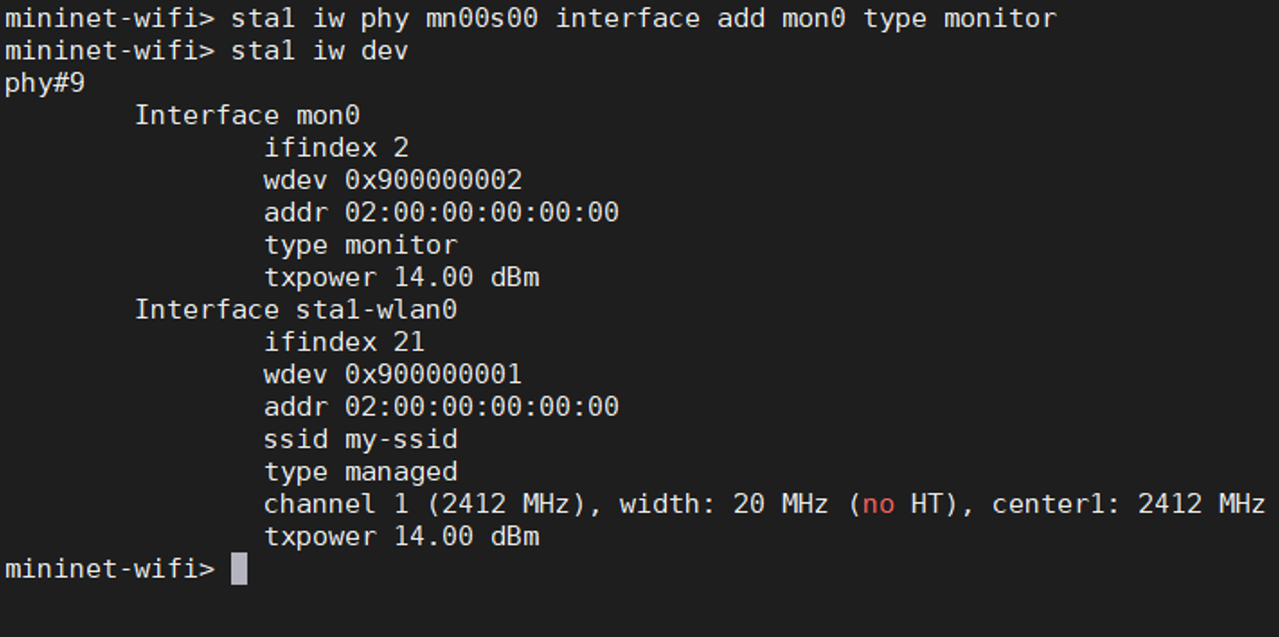
\includegraphics[width=10cm]{archivos/img/conclusiones/future_work2.png}
    \caption{Verificación de la creación de la interfaz en modo monitor.}
    \label{fig:future_monverficacion}
\end{figure}

Acto seguido, según se comentaba, se va a proceder abriendo Wireshark\footnote{\url{https://www.wireshark.org/}} como \textit{sniffer} en la estación WiFi (\textit{sta2}), y se va a generar un único ping desde la estación WiFi (\textit{sta1}). Como se puede apreciar en la figura \ref{fig:future_ping}, llega correctamente el ping al destino, pero como estamos escuchando en una interfaz en modo managed de tipo Ethernet, el Kernel ya ha realizado la traducción de las cabeceras.

\begin{figure}[ht]
    \centering
    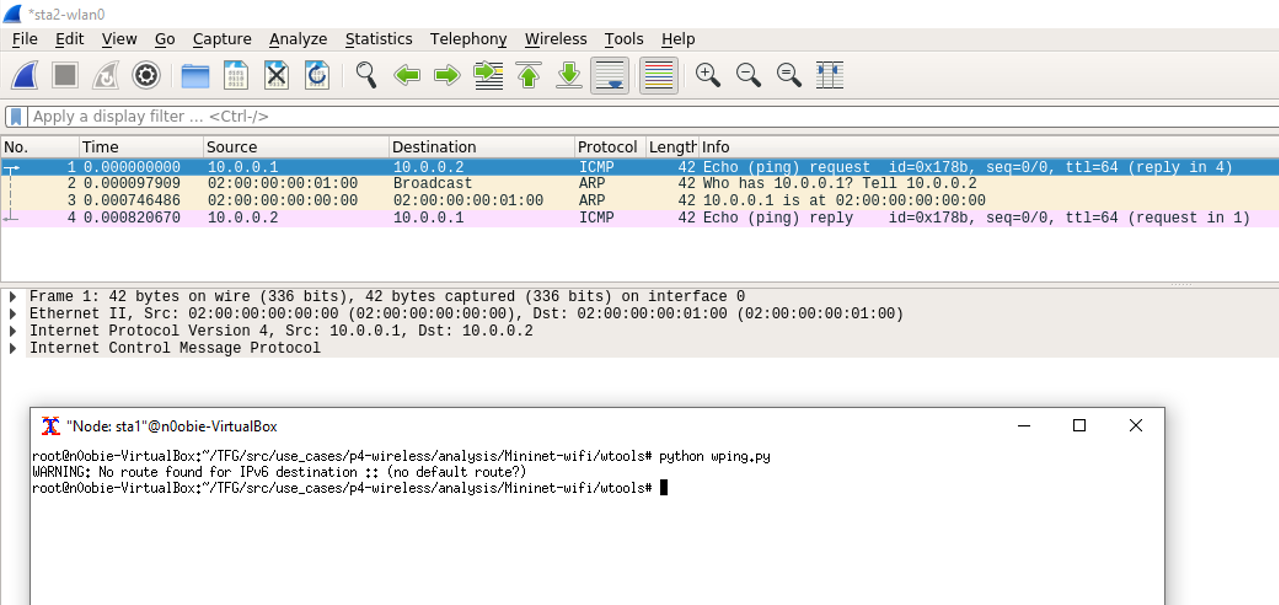
\includegraphics[width=14cm]{archivos/img/conclusiones/wping.png}
    \caption{Generación de ping vía interfaz en modo monitor.}
    \label{fig:future_ping}
\end{figure}

Si se quiere ver con qué cabeceras sale realmente el paquete, se puede realizar una escucha en la interfaz en modo monitor en la cual se está realizando la inyección de paquetes. De esta forma, los paquetes al ser inyectados no se verán afectados por ningún tipo de traducción realizada en el Kernel. En la figura \ref{fig:future_ping_hdrs}, se puede ver como realmente el paquete sale con las cabeceras WiFi indicadas. Además, si nos fijamos en sus direcciones MAC, podemos ver cómo están establecidas, indicando siguiente salto, transmisor, destino final y el origen del ping.
\newpage
\begin{figure}[ht]
    \centering
    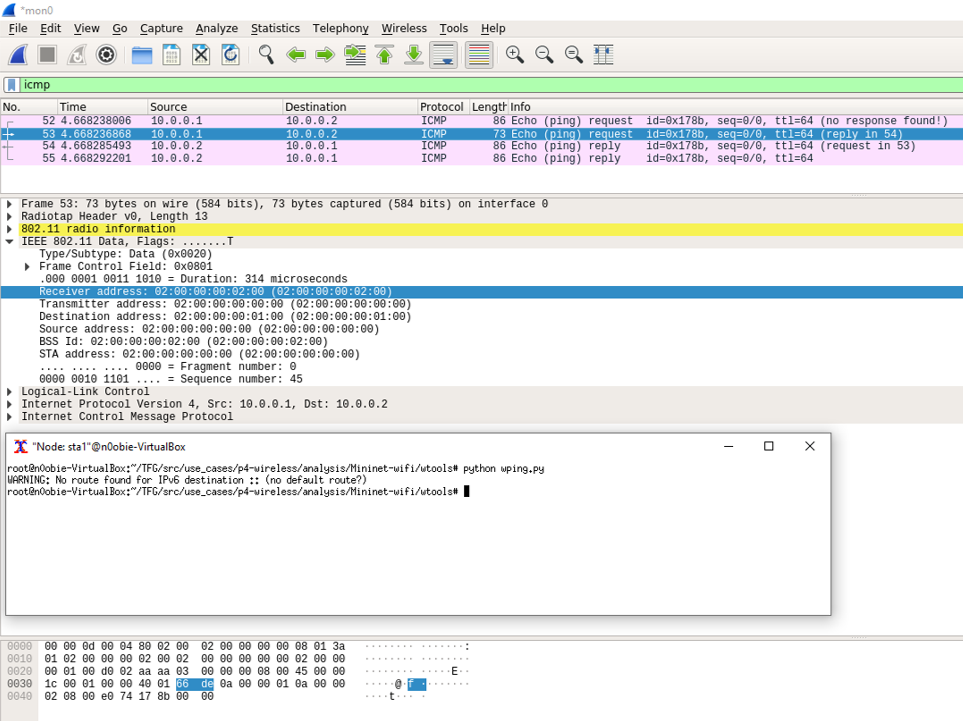
\includegraphics[width=14cm]{archivos/img/conclusiones/wping_hdrs.png}
    \caption{Comprobación de las cabeceras del ping generado vía interfaz en modo monitor.}
    \label{fig:future_ping_hdrs}
\end{figure}

Por lo tanto, se concluye diciendo que sí es viable la transmisión de paquetes a través de interfaces en modo monitor. Como se puede apreciar en la figura \ref{fig:future_ping_hdrs}, hay paquetes presuntamente duplicados, pero si nos fijamos en sus cabeceras se puede ver como dichos paquetes son los paquetes del salto intermedio entre las estaciones WiFi (\textit{sta1} - \textit{ap1} - \textit{sta2}). \\

\par
Esto ocurre debido a que la interfaz monitor hace una escucha pasiva del medio, escuchando todos los paquetes que estén en el rango de la interfaz. Por esto, se propone aplicar un filtrado por MAC destino tanto en \gls{xdp} como en P4 para recibir únicamente los paquetes que van dirigidos a dicha interfaz. De esta modo, se consigue abordar la problemática de transmisión y recepción de paquetes con interfaces creadas con el módulo mac80211\_hwsim en modo monitor, habilitando así la gestión directa de las cabeceras \texttt{ieee80211}.\\
\par

Por consiguiente, se cree que esta vía de trabajo futuro puede ayudar a trabajar más cerca de la tecnología wireless al poder gestionar directamente sus cabeceras y paquetes de control (\textit{beacons}). 

\newpage
%%%%%%%%%%%%%%%%%%%%%%%%%%%%%%%%%%%%%%%%%%%%%%%%%%%%%%%%%%%%%%%%%%%%%%%%%%%%%%%%%%%%%%%%%%%%%%%%%
\subsection{Emulación de redes de baja capacidad - mac802154\_hwsim}

En este punto, se expone una nueva vía de trabajo futuro, en la cual se propone exportar los casos de uso realizados a un entorno más enfocado al \gls{iot}. Por ello, se analizará si es viable exportar los casos de uso realizados anteriormente en medios cableados e inalámbricos bajo el estándar wireless de baja capacidad llamado \texttt{ieee802154}. \\
\par
De esta forma se quiere explorar las fortalezas y debilidades, tanto de \gls{xdp} como del lenguaje P4, en la definición del \textit{datapath} de dispositivos de baja capacidad en un escenario \gls{iot}. Dichos dispositivos, al tener una condición de baja capacidad (estando bastante limitados en batería, alcance, memoria y procesamiento), necesitarán que la tecnología que les defina su \textit{datapath} sea lo más eficiente posible, haciendo un uso optimizado de los recursos de la mota \gls{iot}. Este escenario tan limitado esclarecerá qué tecnología es más idónea a la hora de trabajar en \gls{iot}.

\subsubsection{Herramientas para interactuar con el stack \texttt{ieee802154}}

Se ha empezado analizando qué herramientas de espacio de usuario se tienen disponibles actualmente para trabajar con el subsistema \texttt{ieee802154}. Se encontraron numerosas herramientas y recursos después de ver qué dependencias instala Mininet-WiFi para interactuar con su módulo de \gls{iot}. \\
\par
Todas las herramientas que han sido útiles en este análisis se muestran en la tabla \ref{tab:ieee802154_tools}. Además, se ha incluido un enlace a la pagina oficial de su código fuente, donde se indica cómo instalarlas y cómo hacer uso de ellas.

\vspace{0.5cm}

\begin{table}[ht]
\centering
\resizebox{\textwidth}{!}{%
\begin{tabular}{|l|l|l|}
\hline
\rowcolor[HTML]{EFEFEF} 
\multicolumn{1}{|c|}{\cellcolor[HTML]{EFEFEF}\textbf{Herramienta}} & \multicolumn{1}{c|}{\cellcolor[HTML]{EFEFEF}\textbf{Explicación}}                                                                                                                                                                                                        & \multicolumn{1}{c|}{\cellcolor[HTML]{EFEFEF}\textbf{Enlace}} \\ \hline
\texttt{iwpan}                                                     & \begin{tabular}[c]{@{}l@{}}Herramienta principal para la configuración del subsistema ieee802154, sus interfaces y sus radios. \\ Esta herramienta es muy similar a al herramienta iw pensada para controlar el subsistema Wireless\\  del Kernel de Linux.\end{tabular} & \multicolumn{1}{c|}{\href{https://github.com/linux-wpan/wpan-tools/tree/master/src}{Enlace al código}}                          \\ \hline
\texttt{wpan-hwsim}                                                & \begin{tabular}[c]{@{}l@{}}Herramienta para gestionar el modulo mac802154\_hwsim, permitiendo añadir o eliminar radios, \\ así como añadir enlaces entre distintos radios a través de netlink.\end{tabular}                                                              & \href{https://github.com/linux-wpan/wpan-tools/tree/master/wpan-hwsim}{Enlace al código}                                                 \\ \hline
\texttt{wpan-ping}                                                 & Herramienta para hacer ping directamente con el stack ieee802154.                                                                                                                                                                                                        &  \href{https://github.com/linux-wpan/wpan-tools/tree/master/wpan-ping}{Enlace al código}                                               \\ \hline
\end{tabular}%
}
\caption{Resumen de las herramientas del entorno ieee802154}
\label{tab:ieee802154_tools}
\end{table}

\subsubsection{Arquitectura del stack ieee802154}

A continuación, se expone un diagrama de la arquitectura del stack \texttt{ieee802154}\footnote{\url{https://github.com/linux-wpan/wpan-misc}}, obtenido del repositorio oficial del desarrollo de las herramientas y de los módulos asociados al estándar \texttt{ieee802154} del Kernel de Linux. Este esquema ha sido de gran utilidad para comparar sus distintos bloques con el módulo mac80211\_hwsim\footnote{\url{https://wireless.wiki.kernel.org/en/users/drivers/mac80211_hwsim}}, el cual se utilizó para emular redes inalámbricas bajo el estándar \texttt{ieee80211}.



\begin{figure}
\centering
{\fontsize{5.20}{4}\selectfont 
\begin{verbatim}
              .-------------------------------------------------------------------------------------------------------.
              |                                               Userspace                                               |
              '-----------------^----------------------------------^----------------------------------^---------------'
                                |                                  | socket                           |
                                |                                  v                                  |
                                |                  .------------------------------.                   |
                                | socket           |             IPv6             |                   |
                                |                  '------------------------------'                   | netlink
                                |                                         ^                           |
             .------------------|-----------------------------------------|---------------------------|-----------------.
             |                  |                             ieee802154  |                           |                 |
             |------------------|-----------------------------------------|---------------------------|-----------------|
             |                  v                                         v                           |                 |
             | .---------------------------------. .-----------------------------.                    |                 |
             | |        802.15.4 Sockets         | |      802.15.4 6LoWPAN       |                    |                 |
             | |---------------------------------| |-----------------------------|    .---------------v-------------.   |
             | |.--------------. .--------------.| |                             |    |          nl802154           |   |
             | ||    DGRAM     | |     RAW      || |  .-----------------------.  |    |-----------------------------|   |
             | || data payload | |  full frame  || |  |    Generic 6LoWPAN    |  |    |                             |   |
             | |'------^-------' '--------------'| |  | .-------------------. |  |    |  .----------. .-----------. |   |
             | |       |                | ^      | |  | |        NHC        | |  |    |  |   mlme   | | cmd, etc. | |   |
             | |       |                | |      | |  | '-------------------' |  |    |  |----------| |-----------| |   |
             | |       v                | |      | |  '-------------^---------'  |    |  | assoc.   | | panid     | |   |
             | | .------------.         | |      | |                |            |    |  | deassoc. | | channel   | |   |
             | | | dataframes |       tx| | rx   | |       .--------v--------.   |    |  | ...      | | ...       | |   |
             | | '------------'         | |      | |       |   dataframes    |   |    |  '----------' '-----------' |   |
             | |     |    ^             | |      | |       '-------^-|-------'   |    |       |             ^       |   |
             | '-----|----|-------------|-|------' '---------------|-|-----------'    |       |             |       |   |
             |       |    |             | |-----------.            | |                |       |             |       |   |
             |    tx |    |rx           '-------|     |            | |                '-------|-------------|-------'   |
             |       |    |---------------------|-----|------.   rx| |tx                      |             |           |
             |       v                          |     |      |     | |                        |             |           |
             | .------------------------------. |     |      |     | |                        |             |           |
             | |        frame creation        | |     |      |     | |                        |             |           |
             | |------------------------------| |     |      |     | |                        |             |           |
             | | generic functions            <-|-----|--------------'                        |             |           |
             | | - wpan_dev callbacks struct? | |     |      |     |                          |             |           |
             | |   instead dev_hard_header    | |     |      |     |   .-------------------.  |             |           |
         ******|   different HardMAC/SoftMAC  | |     |      |     |   |  mlme operations  |  |             |           |
         *   | | - data                       | |     |      |     |   |                   |<-'             |           |
         *   | | --- for mlme ---             | |     |      |     |   '-------------------'                |           |
         *   | | - beacon                     | |     |      |     |                |                       |           |
         *   | | - cmd                        | |     |      |     |                |                       |           |
         *   | | - ack? -> (slotted mode)     | |     |      |     |                |                       |           |
         *   | '--------------|---------------' |.-------------------------.        |                       |           |
         *   |                v                 ||  802.15.4 packet_layer  |        |             ----------'           |
         *   |       .----------------.         |'-------------------------'        |             |                     |
         *   |       | dev_queue_xmit |<--------'            ^                      |             |                     |
         *   |       '----------------'                      |                      |             |                     |
         *   '----------------|------------------------------|----------------------|-------------|---------------------'
         *              .-----|------------------------------|----------------------|-------------|------------.
         *              |     |                              | mac802154            |             |            |
         *              |-----|------------------------------|----------------------v-------------v------------|
         *              |     |                              |               .-------------..-----------.      |
         *******************************************************************>| do mlme ops || cfg802154 |      |
can use frame creation  |     |   .--------------------------|-------------. '-------------'|-----------|      |
                        |     |   | Frame parsing (call netif_receive_skb) |        |       | panid     |--------|
                        |     |   |----------------------------------------|        |       | shortaddr |      | |
                        |     |   | again check if 802.15.4 compliant      |        |       | etc.      |      | |
                        |     |   | different handling coordinator/node    |        |       '-----------'      | |
                        |     |   | set packet type (e.g. PACKET_HOST)     |        |                          | |
                        |     |   '---------------------^------------------'        |                          | |
                        |     |                         |                           | tx workqueue             | |
                        |     |ndo_start_xmit           |   |-----------------------'                          | |  .--------------.
                        |     |      .------------------|---|--------------------------------------.           | |  | e.g. tcpdump |
                        |     |      |                  |   |interface types                       |           | |  '--------------'
                        |     |      |------------------|---|--------------------------------------|           | |          ^
                        |     |      |                  |   |                                      |           | |          |
                        |     |      | .----------------|---v-----------.  .---------------------. |           | |          |
                        |     |      | |             frames             |  |       frames        | | mac sett. | |    .-----------.
                        |     '-------->    for rx, filtered by phy     |  | non-filtered by phy | |<------------|    | af_packet |
                        |            | |--------------------------------|  |---------------------| |           | |    '-----------'
                        |        .---| |                                |  |                     |----.        | |          ^
                        |        |   | | .-------------.  .-----------. |  | .-----------.       | |  |        | |          |
                        |        |   | | | coordinator |  |   node    | |  | |  monitor  |-----------------------|----------'
                        |        |   | | '------^------'  '-----^-----' |  | '-----------'       | |  |        | |
                        |        |   | '--------|---------------|-------'  '-------^-------------' |  |        | |
                        |        |   '----------|---------------|------------------|---------------'  |        | |
                        |        |              | rx/tx         | rx/tx            |rx/tx not possible(no AACK)| |
                        |        |              |               |         |--------|                  |        | |
                        '--------|--------------|---------------|---------|--------|------------------|--------' |
                                 |              v               v         |        |                  |          |
                                 |         ===================================     |                  |          |
                                 |               ^          ^          ^           |                  |          |
                                 |        .------|----------|----------|-----------|------.           |          |
    each interface type has      |        |      |          |  Frames  |           |      |           |     if AACK, ack frames are handled   
    different phy address filters|        |------|----------|----------|-----------|------|           |     by phy layer, not driver.         
    - sets mac settings on ifup  |        | .----v----..----v----..----v----. .---------. |  AACK ----|--->                                   
                                 |        | |  data   ||   cmd   || beacon  | |   ack   |------.      |     AACK disabled if promiscuous mode.
                                 |        | '----^----''----^----''----^----' '----^----' |    |      |     Then driver receives ack frames.  
                                 |        '------|----------|----------|-----------.------'    |      |          |
                                 |               |          |          |           .           |      |          |
                                 |               |          |          |           .           |      | sets promiscuous mode
                                 |        .------v----------v----------v-----------v------.    |      |          |
                                 |        |            802.15.4 SoftMAC Driver            |    |      |          |
                                 |        |-----------------------------------------------|    |      |          |
                                 |        | - supports always AACK handling               |    |      |          |
                                 -------->|   - ACK handling is done by phy (AACK)        |<-----------          |
                                          |   - on AACK, ACK frames doesn't reach driver  |<----------------------
                                          | - filtering (CRC, address, what phy can do..) |    |   phy settings
                                          '-----------------------------------------------'    |
                                                                  ^                            |
                                                                  |                            |
                                                                  v                            |
                                                      .----------------------.                 |
                                                      | 802.15.4 SoftMAC PHY |<----------------'
                                                      '----------------------'
\end{verbatim}
}
\caption{Arquitectura del stack \texttt{ieee802154} \cite{wpanArch}}
\label{fig:arch_ieee802154}
\end{figure}


\newpage

Tras analizar la arquitectura es posible ver que este módulo, a diferencia del módulo mac80211\_hwsim, no conecta a la capa física (\textit{phy}) interfaces del tipo Ethernet. Es importante recordar que cuando se trabaja con WiFi se estudió por qué se hacía un parseo de paquetes con cabeceras 802.11 hacia cabeceras 802.3 y viceversa en el Kernel.\\
\par

Al generalizar hacia interfaces Ethernet, las aplicaciones que trabajan a nivel de interfaz son muy extrapolables, ya que pueden ser portadas a distintos tipos de dispositivos con distintas características. Es verdad que se pierde en rendimiento, ya que el paquete se encola hasta tres veces en el Kernel y requiere procesamiento adicional, pero por otro lado se gana muchísima versatilidad.

\subsubsection{Viabilidad de los casos de uso}

 Teniendo en cuenta que no se emplean interfaces de Ethernet para comunicar la capa física con las capas superiores, los casos de uso no serían extrapolables de forma inmediata, ya que en las etapas de parseo de todos los casos de uso, se parseaba a una cabecera del tipo Ethernet, tanto en \gls{xdp} haciendo accesos a memoria, como en P4 con las distintas etapas de \textit{parsing}.\\
\par

Por tanto, en vez de parsear los paquetes hacia estructuras de Ethernet, habría que hacerlo hacia estructuras que definieran la estructura de la cabecera \texttt{ieee802154}. Se ha buscando en el \href{https://elixir.bootlin.com/linux/latest/source/include/net/ieee802154_netdev.h}{Kernel}, donde se ha encontrado que dicha estructura ya está definida, por lo que solo habría que hacer uso de ella en los casos de uso de \gls{xdp}, y en los casos de uso de P4 habría que declarar la estructura análoga y sustituir el parser de Ethernet por el parser de cabeceras 802.15.4. 

\begin{lstlisting}[language=C, style=C-color, caption={Estructura para manejar paquetes de l estándar ieee802154},label=code:futureW_ieee802154hdr]
    struct ieee802154_hdr {
    	struct ieee802154_hdr_fc fc;
    	u8 seq;
    	struct ieee802154_addr source;
    	struct ieee802154_addr dest;
    	struct ieee802154_sechdr sec;
    };
\end{lstlisting}

\vspace{0.5cm}
No obstante, aunque la vía de trabajo futuro ya se encuentra bien definida, se va a realizar una prueba de concepto probando a añadir un programa \gls{xdp} a una interfaz generada por el módulo mac802154\_hwsim. De este modo, se quiere consolidar esta vía de trabajo futuro probando que si admite soporte para \gls{xdp}.\\
\par
En cuanto a el \gls{bmv2}, se entiende que no debe suponerle un problema hacer uso de las interfaces suministradas, ya que este hace uso de la librería \href{https://github.com/p4lang/behavioral-model/blob/master/src/BMI/bmi_interface.c}{\textbf{libpcap}} para gestionar el envío y recepción de los paquetes. Esta librería se ha visto que hace uso de la interfaz de sockets en última instancia, se puede ver \href{https://github.com/the-tcpdump-group/libpcap/blob/master/pcap.c}{\textbf{aquí}} en el código fuente, por lo que no supondría ninguna incompatibilidad con la arquitectura de subsistema \texttt{ieee802154} que admite la operabilidad con distintas familias de sockets.


\subsubsection{Carga de programas \glsentryshort{xdp} en interfaces \texttt{ieee802154}}

 Como ya se ha comentado, la viabilidad de replicar los casos de uso sobre el módulo mac802154\_hwsim pasa por si el stack \texttt{ieee802154} es capaz de gestionar la carga de programas \gls{xdp} en sus interfaces. Por otro lado, como ya se había mencionado con el \gls{bmv2} no habría ningún problema ya que iría sobre la interfaz de sockets del Kernel, por lo que la arquitectura del propio módulo lo contempla. \\
\par

Se ha buscado información al respecto sobre si el modulo era compatible con la carga de programas \gls{bpf}, que al final es en lo que se traduce un programa \gls{xdp}, pero no se ha encontrado información precisa al respecto, por lo que se ha decidido hacer una prueba de concepto de carga de programas \gls{xdp}. Como se comentó previamente, los programas \gls{xdp} no son extrapolables directamente al subsistema \texttt{ieee802154}, por esto se hará uso del \href{https://github.com/davidcawork/TFG/tree/master/src/use_cases/xdp/case01}{\textbf{case01}} donde únicamente se implementaba una funcionalidad del \textit{datapath} haciendo uso de los códigos de retorno \gls{xdp}.\\
\par


De esta forma no será necesario parsear las cabeceras \texttt{ieee802154}, y se podrá ver de una forma rápida si dichas interfaces asociadas a los radios con la capa física \texttt{ieee802154} SoftMAC soportan la carga de un programa \gls{xdp} genérico. Esta prueba en primera instancia, se hizo directamente cargando el módulo y creando las interfaces pero, ya que Mininet-WiFi da soporte\footnote{\url{https://github.com/intrig-unicamp/mininet-wifi/tree/master/mn_wifi/sixLoWPAN}} para gestionar dicho módulo a través de la implementación de Mininet-IoT, se pensó que daría cierta continuidad el desarrollo de los distintos casos de uso en dicha herramienta de emulación. \\

\par

A partir de este punto solo puede continuar si se posee una versión del Kernel \texttt{v4.18.x} o superior, ya es a partir de esta donde se incluye el módulo mac802154\_hwsim. Lo primero que se hará es volver a la instalación de Mininet-WiFi donde se llevarón a cabo los casos de uso wireless, e instalar las dependencias necesarias para la gestión del módulo mac802154\_hwsim. 

\begin{lstlisting}[language= bash, style=Consola, caption={Instalación de las dependencias de Mininet-WiFi - mac802154\_hwsim},label=code:futureW_installdeps6]
    # Entramos en el directorio de mininet-wifi
    cd mininet-wifi
    
    
    # Añadimos las dependencias para la gestión del módulo mac802154_hwsim
    sudo util/install.sh -6

\end{lstlisting}
\vspace{0.5cm}

Ahora con las dependencias ya añadidas, vamos a se va hacer uso del ejemplo que utiliza el módulo mac802154\_hwsim disponible en Mininet-WiFi, para probar la carga del programa \gls{xdp} desarrollado en el \href{https://github.com/davidcawork/TFG/tree/master/src/use_cases/xdp/case01}{\textbf{case01}}. Dicho ejemplo puede ser encontrado bajo el directorio \texttt{examples} con el nombre de \texttt{6LoWPan.py}. Cabe mencionar que en este ejemplo se añade una interfaz auxiliar que añade la capa de gestión del estándar 6LoWPan\footnote{\url{https://tools.ietf.org/html/rfc8138}}. En este caso, esta interfaz auxiliar es irrelevante, ya que la carga del programa se hará sobre la interfaz nativa de subsistema \texttt{ieee802154}.

\begin{lstlisting}[language= bash, style=Consola, caption={Ejecución ejemplo 6LoWPan.py},label=code:futureW_run6]
    # Entramos al directorio de los ejemplos
    cd examples
    
    # Ejecutamos el ejemplo
    sudo python 6LoWPan.py
\end{lstlisting}

\vspace{0.5cm}

Una vez cargado el ejemplo, se tendrá la CLI de Mininet-WiFi abierta, y lo siguiente que se hará será compilar el caso de uso \gls{xdp}. Como ya comentamos anteriormente, será el \href{(https://github.com/davidcawork/TFG/tree/master/src/use_cases/xdp/case01}{\textbf{case01}}.

\begin{lstlisting}[language= bash, style=Consola, caption={Compilación del programa XDP - mac802154\_hwsim},label=code:futureW_com6]
    # Nos movemos de directorio y compilamos el case01
    mininet-wifi> sh cd ~/TFG/src/use_cases/xdp/case01 && sudo make

\end{lstlisting}

\vspace{0.5cm}

 Ya se tendría compilado el caso de uso \gls{xdp} y listo para ser cargado sobre la interfaz. Pero, se debe plantear la siguiente cuestión ¿Sobre qué interfaz se debe cargar el programa \gls{xdp}? Bien, para contestar esta pregunta se debe inspeccionar antes las interfaces de uno de los sensores que hay en la topología del ejemplo.\\
 \par
 Como los sensores corren en su propia \textit{Network namespace}, se tendrá tendremos que abrir una xterm o indicar el nombre de nodo previamente en la CLI de Mininet-WiFi para que dicho comando se ejecute dentro de la \textit{Network Namespace} indicada.

\begin{lstlisting}[language= bash, style=Consola, caption={Obtención de interfaz 802.15.4},label=code:futureW_intf6]
    mininet-wifi> sensor1 ip a s
        1: lo: <LOOPBACK,UP,LOWER_UP> mtu 65536 qdisc noqueue state UNKNOWN group default qlen 1000
            link/loopback 00:00:00:00:00:00 brd 00:00:00:00:00:00
            inet 127.0.0.1/8 scope host lo
              valid_lft forever preferred_lft forever
            inet6 ::1/128 scope host
              valid_lft forever preferred_lft forever
        2: sensor1-pan0@sensor1-wpan0: <BROADCAST,MULTICAST,UP,LOWER_UP> mtu 1280 qdisc noqueue state UNKNOWN group default qlen 1000
            link/6lowpan 9e:7b:c7:68:bb:9c:31:56 brd ff:ff:ff:ff:ff:ff:ff:ff
            inet6 2001::1/64 scope global
              valid_lft forever preferred_lft forever
        248: sensor1-wpan0: <BROADCAST,NOARP,UP,LOWER_UP> mtu 123 qdisc fq_codel state UNKNOWN group default qlen 300
            link/ieee802.15.4 9e:7b:c7:68:bb:9c:31:56 brd ff:ff:ff:ff:ff:ff:ff:ff
    

\end{lstlisting}

\vspace{0.5cm}
Como se puede apreciar en el bloque \ref{code:futureW_intf6} la interfaz que añade la capa 6LoWPan es la interfaz \texttt{sensor1-pan0}, por lo tanto unicamente se hara uso de la interfaz que comunica de forma directa con el subsistema \texttt{ieee802154}. De forma adicional, se puede utilizar la herramienta \texttt{iwpan}, mencionada en la sub-sección de herramientas del stack ieee802154, para ver qué interfaces (\textit{dev}) están disponibles y sobre qué radio están conectadas según se puede ver en el bloque \ref{code:futureW_intf26}.

\begin{lstlisting}[language= bash, style=Consola, caption={Obtención de interfaz 802.15.4 haciendo uso de la herramienta iwpan},label=code:futureW_intf26]
    mininet-wifi> sensor1 iwpan dev
        phy#24
                Interface sensor1-wpan0
                        ifindex 248
                        wpan_dev 0x1800000002
                        extended_addr 0x9e7bc768bb9c3156
                        short_addr 0xffff
                        pan_id 0xbeef
                        type node
                        max_frame_retries 3
                        min_be 3
                        max_be 5
                        max_csma_backoffs 4
                        lbt 0
                        ackreq_default 0
        

\end{lstlisting}

\vspace{0.5cm}

 Por tanto, una vez que se sabe sobre qué interfaz operar (en este caso se trabajará sobre el sensor1 en la interfaz \texttt{sensor1-wpan0}), solo queda cargar el programa y ver si realmente soporta la funcionalidad del mismo.

%\todo{Cambiar este bloque de código por una imagen ya que es un resultado}
\begin{lstlisting}[language= bash, style=Consola, caption={Carga de programa XDP en interfaz ieee802154},label=code:futureW_load6]
    mininet-wifi> sensor1 cd /home/n0obie/TFG/src/use_cases/xdp/case01
    mininet-wifi> sudo ./xdp_loader -S -d sensor1-wpan0 -F --progsec xdp_case01
        Success: Loaded BPF-object(prog_kern.o) and used section(xdp_case01)
         - \gls{xdp} prog attached on device:sensor1-wpan0(ifindex:248)
         - Pinning maps in /sys/fs/bpf/sensor1-wpan0/
    mininet-wifi>
\end{lstlisting}
\vspace{0.5cm}
Se puede ver como el programa ha sido correctamente cargado en la interfaz. Además, los mapas se anclaron de manera satisfactoria en sistema de archivos \gls{bpf} por lo que se habilita la recolección de estadísticas relativas a los códigos de retorno \gls{xdp}. \\
\par
Para la comprobación de la funcionalidad del programa \gls{xdp}, se llevará a cabo un ping entre los dos sensores, ya que al implementar un código de retorno \texttt{XDP\_DROP} no habrá conectividad entre ellos.
%\todo{Cambiar este bloque de código por una imagen ya que es un resultado}
\begin{lstlisting}[language= bash, style=Consola, caption={Comprobación funcionamiento programa XDP en interfaz ieee802154},label=code:futureW_func6]
    # Ojo! Con el programa XDP cargado en la interfaz
    mininet-wifi> sensor1 ping sensor2
    PING 2001::2(2001::2) 56 data bytes
    From 2001::1 icmp_seq=1 Destination unreachable: Address unreachable
    From 2001::1 icmp_seq=2 Destination unreachable: Address unreachable
    From 2001::1 icmp_seq=3 Destination unreachable: Address unreachable
    ^CsendInt: writing chr(3)
    
    --- 2001::2 ping statistics ---
    4 packets transmitted, 0 received, +3 errors, 100% packet loss, time 3072ms
    
    mininet-wifi>

\end{lstlisting}

\newpage

 Como se puede apreciar el comportamiento es el esperado, pero aun así, cabría pensar que la falla de conectividad entre ambos sensores es debida a otra razón, por ello se va eliminar el programa \gls{xdp} de la interfaz y se va a probar de nuevo la conectividad entre ambos sensores.
%\todo{Cambiar este bloque de código por una imagen ya que es un resultado}
\begin{lstlisting}[language= bash, style=Consola, caption={Comprobación de funcionamiento del programa XDP - 2},label=code:futureW_func26]
    # Quitamos el programa XDP de la interfaz 
    mininet-wifi> sensor1 cd /home/n0obie/TFG/src/use_cases/xdp/case01 
    mininet-wifi> sudo ./xdp_loader -S -U -d sensor1-wpan0
    INFO: xdp_link_detach() removed XDP prog ID:677 on ifindex:248
    mininet-wifi>
    
    
    # Probamos de nuevo la conectividad entre ambos sensores
     mininet-wifi> sensor1 ping sensor2
    PING 2001::2(2001::2) 56 data bytes
    64 bytes from 2001::2: icmp_seq=1 ttl=64 time=0.053 ms
    64 bytes from 2001::2: icmp_seq=2 ttl=64 time=0.044 ms
    64 bytes from 2001::2: icmp_seq=3 ttl=64 time=0.044 ms
    64 bytes from 2001::2: icmp_seq=4 ttl=64 time=0.106 ms
    ^CsendInt: writing chr(3)
    
    --- 2001::2 ping statistics ---
    4 packets transmitted, 4 received, 0% packet loss, time 3049ms
    rtt min/avg/max/mdev = 0.044/0.061/0.106/0.027 ms
    mininet-wifi>

\end{lstlisting}

\vspace{0.5cm}

 Teniendo en cuenta todos los aspectos que se han comentado en este análisis de viabilidad sobre esta vía de trabajo futuro, se concluye diciendo que los casos de uso no son extrapolables directamente, ya que las interfaces no son del tipo Ethernet. Esto implicaría rehacer el módulo de \textit{parsing} de capa dos, algo admisible y factible. \\
\par

 Por tanto, se propone a futuro llevar a cabo dicho desarrollo, además de estudiar y analizar distintas variables que entran en juego en un entorno inalámbrico de baja capacidad. Como son la batería, la memoria, el numero de transmisión y recepciones, entre otras. De esta forma se podrá concluir qué tecnología, si P4 ó \gls{xdp}, nos permitirá programar dispositivos \gls{iot} con una mayor eficiencia en redes 802.15.4.


